\documentclass[tikz,border=7pt]{standalone}
\begin{document}
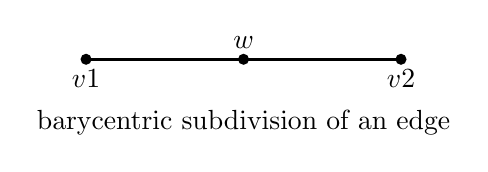
\begin{tikzpicture}[line width=.9pt]
\coordinate (v1) at (-2,0); \coordinate (v2) at (2,0); \coordinate (w) at (0,0);
\draw (v1)--(w)--(v2); \foreach \p/\pos in {v1/below,v2/below,w/above} \fill (\p) circle (2pt) node[\pos] {$\p$};
\node at (0,-.8) {barycentric subdivision of an edge};
\end{tikzpicture}
\end{document}
